\documentclass[11pt]{exam}
\usepackage[margin=1in]{geometry}
\pagestyle{plain}
\usepackage{amsmath,amsfonts,amssymb,amsthm,enumerate}
\usepackage{multicol}
\usepackage[]{graphicx}
\usepackage{hyperref}
\usepackage{tikz}
\usepackage{pgfplots}
\usepackage{subfigure}
\usepackage[final]{pdfpages}

\newcommand{\dydx}{\frac{dy}{dx}}
\newcommand{\dxdy}{\frac{dx}{dy}}

\addtolength{\footskip}{2\baselineskip} % to lower the page numbers
\title{\vspace{-0.5in} Math 115 \\ Worksheet Section 3.7}
\date{}


% \theoremstyle{definition}
% \newtheorem{problem}{Problem}
\renewcommand{\questionlabel}{\textbf{Problem~\thequestion.}}
%\printanswers

\begin{document}
\maketitle
\vspace{-0.75in}
\begin{questions}
\question
  \begin{enumerate}[(a)]
	\item Find $\displaystyle\frac{dy}{dx}$ given that $x^2 + y^2 - 4x + 7y = 15$.
          \vspace{0.2in}
	\item Under what conditions on $x$ and/or $y$ is the tangent line to this curve horizontal? 
          \vspace{0.2in}
        \item Find $\displaystyle\frac{dx}{dy}$ (pay attention to the order!)
          \vspace{0.2in}
        \item Under what conditions on \(x\) and/or \(y\) is the
          tangent line to this curve vertical?
  \end{enumerate}
  \begin{solution}
    Throughout, we must remember that \(y\) and \(x\) are implicitly
    related, so we have to use the chain rule.
    \begin{enumerate}
    \item Differentiating both sides with respect to \(x\) gives us \(2x + 2y\dydx - 4 + 7
      \dydx = 0\). We then solve
      \begin{align*}
        2x + 2y\dydx - 4 + 7
        \dydx = 0 & \implies (2y+7)\dydx = 4-2x \\
        & \implies \dydx = \frac{4-2x}{2y+7}
      \end{align*}
    \item In this case, \(\dydx = 0 \iff x = 2\).
    \item Differentiating both sides with respect to \(y\) gives us
      \(2x \dxdy + 2y - 4 \dxdy + 7 = 0\). We then solve
      \begin{align*}
        2x \dxdy + 2y - 4 \dxdy + 7 = 0
        & \implies (2x-4) \dxdy = -(2y+7) \\
        & \implies \dxdy = \frac{2y+7}{4-2x}
      \end{align*}
    \item In this case, \(\dxdy = 0 \iff y = -\frac{7}{2}\).
    \end{enumerate}
  \end{solution}
          \vspace{0.2in}
  \question Find $dy/dx$ for $e^{\cos(y)} = x^3\arctan(y)$.
    \begin{solution}
      Differentiating both sides with respect to \(y\), we will have
      to make use of the chain rule on the left hand side and product
      rule on the right hand side. We get \[
        e^{\cos(y)} \cdot (-\sin(y)) \cdot \dydx = 3x^2 \arctan(y) +
        x^3\left( \frac{1}{1+y^2} \right) \cdot \dydx
      \]
      Solving for both sides, we get
      \begin{align*}
        & e^{\cos(y)} \cdot (-\sin(y)) \cdot \dydx = 3x^2 \arctan(y) +
        x^3\left( \frac{1}{1+y^2} \right) \cdot \dydx\\
        & \implies -\left(\sin(y)e^{\cos(y)} + \frac{x^3}{1+y^2}
        \right) \dydx = 3x^2 \arctan(y) \\
        &\implies \dydx = -\frac{3x^2 \arctan(y)}{\sin(y)e^{\cos(y)} + \frac{x^3}{1+y^2}}
      \end{align*}
    \end{solution}
    \vspace{0.1in}
  \question Consider the curve given by the equation $e^{y^2}=x^3 + 9$.
    \begin{parts}
    \part Find $\frac{dy}{dx}$.
    \part Find the coordinates of the two points on the curve where the tangent line is horizontal.
    \part Find any points on the curve where there is a vertical tangent line.
    \end{parts}
    \begin{solution}
      \begin{enumerate}[(a)]
      \item \(e^{y^2} (2y) \dydx = 3x^2 \implies \dydx = \frac{3x^2}{2ye^{y^2}}\)
      \item The tangent line on the curve is horizontal when \(\dydx =
        0 \implies x = 0\). We then solve
        \begin{align*}
          e^{y^2} = 9 & \implies y^2 = \ln(9) \\
          & \implies y = \pm \sqrt{\ln(9)}
        \end{align*}
        Thus, the two points are \((0,\sqrt{\ln(9)})\) and \((0,-\sqrt{\ln(9)})\).
      \end{enumerate}
    \end{solution}
  \question Valerie is building a square chicken coop with side length $x$.  Because she needs a separate place for the rooster, she needs to put fence around the square and also along the diagonal line shown.  The fence costs \$20 per linear meter, and she has a budget of \$900.  

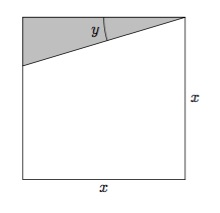
\includegraphics[width=2in]{Figures/coop.jpg}

\vspace*{-2cm}

$$80x + \frac{20x}{\cos(y)}=900$$
\begin{enumerate}[(a)]

\item Verify that the equation above gives the relationship between $x$ and the angle $y$ (in radians).

\vfill


\item If Valerie builds the coop with $y=\pi/6$ (and wants to use her whole budget), find the side length $x$.

\vfill

\item Find slope of the curve at this point, and interpret what it tells Valerie.

\vfill

\end{enumerate}
\begin{solution}
  \begin{enumerate}[(a)]
  \item The perimeter of the square is \(4x\), so the outer fencing
    will cost \(20 \cdot 4x = 80x\). The right triangle above
    satisfies the relationship that \(\cos(y) = \frac{x}{h}\) for
    \(h\) the hypotenuse of the right triangle. Since \(h\) is the
    extra fencing on the inside, we set \(h = \frac{x}{\cos(y)}\) and
    so the cost of that fencing is \(\frac{20x}{\cos(y)}\). So, if she
    has a budget of \(\$900\), then the relationship makes sense.
  \item We solve
    \begin{align*}
      80x + \frac{20x}{\cos(\pi/6)} = 900
      & \implies 80x + \frac{20}{\sqrt{3}/2} x = 900 \\
      & \implies \left(80+\frac{40}{\sqrt{3}}\right) x = 900 \\
      & \implies x = \frac{900}{80+\frac{40}{\sqrt{3}}} \approx 8.73
        \text{ meters}
    \end{align*}
  \item Differentiating both sides with respect to \(x\), we get \begin{align*}
      80 + \frac{20\cos(y)-20x(-\sin(y))\dydx}{(\cos(y))^2} = 0
      & \implies \frac{20x\sin(y)\dydx}{(\cos(y))^2} =
      -80-\frac{20}{\cos(y)} \\
      & \implies \dydx = - \frac{80\cos^2(y)+20\cos(y)}{20x\sin(y)} 
    \end{align*}
    Now, evaluating at the point
    \(\left(\frac{900}{80+\frac{40}{\sqrt{3}}}, \frac{\pi}{6}
    \right)\), we get \[
      \dydx = -
      \frac{80\cos^2(\pi/6)+20\cos(\pi/6)}{20\left(\frac{900}{80+\frac{40}{\sqrt{3}}}\right)\sin(\pi/6)}
      = -\frac{80\cdot \frac{3}{4} + 20 \frac{\sqrt{3}}{2}}{20
        \left(\frac{900}{80+\frac{40}{\sqrt{3}}}\right) \cdot \frac{1}{2}}
      \approx -0.79
    \]
    This tells us that, if Valerie increases the side length \(x\)
    from \(8.73\) meters to \(8.83\) meters, she will have to
    decrease the angle of \(y\) by approximately \(0.079\) radians to
    stay in budget.
  \end{enumerate}
\end{solution}
\pagebreak
\question (Winter 2018 Exam 2) %problem 2
   Find $\displaystyle\frac{dy}{dx}$ for the implicit function given by
   $$2^{x+y} + \sin(x) \cos(y) = 5-x.$$
   \begin{solution}
     See part (b) of \href{https://dhsp.math.lsa.umich.edu/exams/115exam2/w18/s2.pdf}{https://dhsp.math.lsa.umich.edu/exams/115exam2/w18/s2.pdf}
   \end{solution}
   \vspace{0.1in}
\question (Fall 2016 Exam 2) Let $a$ and $b$ be constants. Consider the curve $\mathcal{C}$ defined by the equation
\[
\cos(ax)+by\ln(x)=3+y^3.
\]
Find the formula for $\frac{dy}{dx}$ in terms of $x$ and $y$. The constants $a$ and $b$ may appear in your answer. 
\begin{solution}
  See \href{https://dhsp.math.lsa.umich.edu/exams/115exam2/f16/s10.pdf}{https://dhsp.math.lsa.umich.edu/exams/115exam2/f16/s10.pdf}
\end{solution}
\vspace{0.1in}
\question The folium of Descartes (a.k.a. Descartes' leaf) was first discovered in 1638 and is defined as the curve
\begin{equation*}
	x^3+y^3=6xy.
\end{equation*}
The curve forms a loop in the first quadrant, and it is symmetric
about $y=x$:
\begin{figure}[h]
\centering
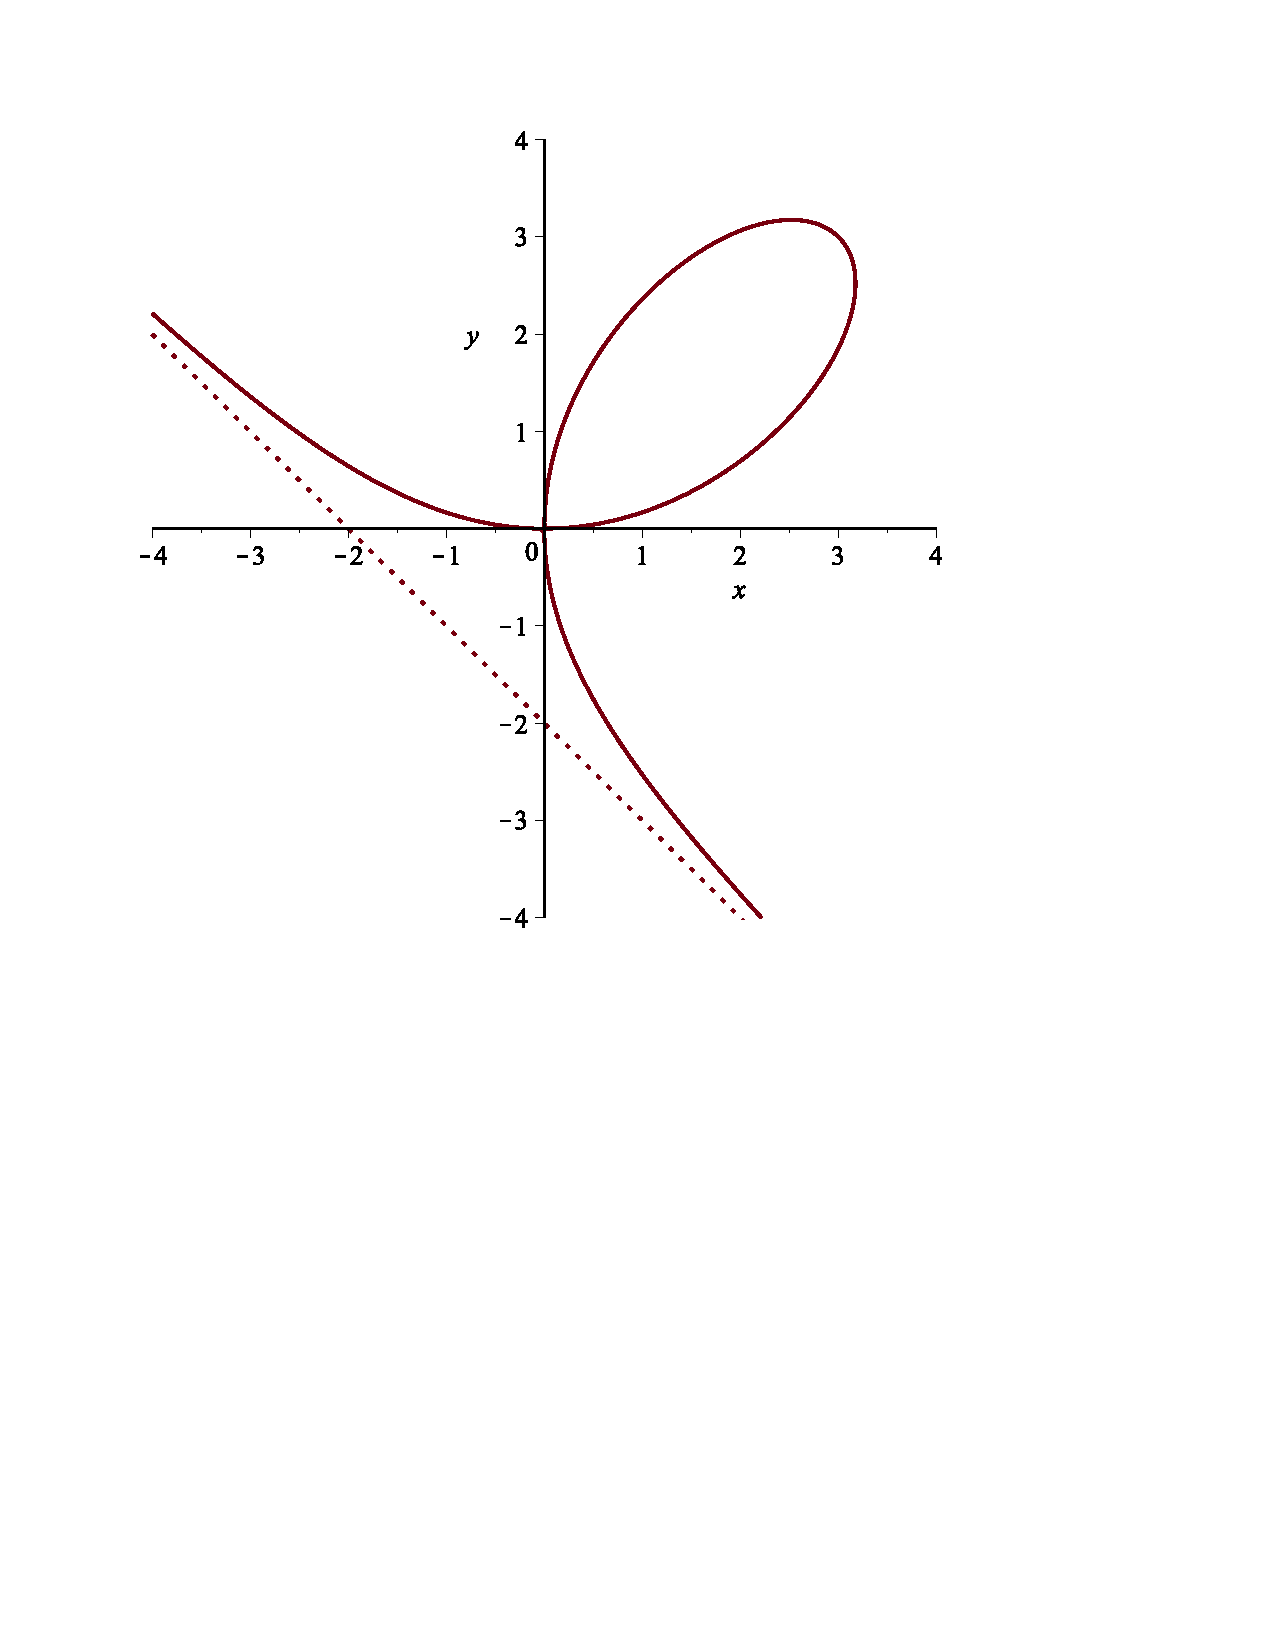
\includegraphics[width=10cm,height=10cm]{Figures/fig1.pdf}
\end{figure}
\begin{enumerate}[(a)]
	\item Show that the point $(x,y)=(3,3)$ lies on the curve.
	\item Find the equation of the tangent line to the curve at the point $(x,y)=(3,3)$.
	\item For what value(s) of $x$ (if any) will the tangent line to this curve be horizontal?
 \end{enumerate}
 \begin{solution}
   \begin{enumerate}[(a)]
   \item We check \(3^3+3^3 = 27+27 = 54 = 6 \cdot 3 \cdot 3\).
   \item We differentiated both sides with respect to \(x\) to get
     \begin{align*}
       3x^2 + 3y^2 \dydx = 6y+6x\dydx
       & \implies (3y^2-6x)\dydx = 6y-3x^2 \\
       & \implies \dydx = \frac{6y-3x^2}{3y^2-6x}
     \end{align*}
     Then, we plug in \(x = 3\) and \(y=3\) to get \[
       \dydx \rvert_{(3,3)} = \frac{6 \cdot 3 - 3 \cdot 3^2}{3 \cdot 3^2-6
         \cdot 3} = -1
     \]
     Thus, the tangent line has slope \(-1\) and passes through the point
     \((3,3)\), so the equation is \[
       y = -(x-3)+3 = -x+6
     \]
     \item The tangent line is horizontal when \(6y-3x^2 = 0 \implies
       y = \frac{1}{2}x^2\) but \(3y^2-6x \neq 0\). Plugging this back into the original
       equation for the folium, we check
       \begin{align*}
         x^3 + \frac{1}{8} x^6 = 3x^3
         & \implies x^3(\frac{1}{8}x^3-2) = 0\\
         & \implies x^3 = 0 \text{ or } \frac{1}{8}x^3-2 = 0 \\
         &  \implies x = 0 \text{ or } x^3 = 16 \\
         &  \implies x = 0 \text{ or } x = 16^{1/3} \approx 2.52\\
       \end{align*}
       However, \(x=0\) is not a solution because this violates the
       condition that \(3y^2-6x \neq 0\). We see this on the picture
       since there is no clear tangent line at the point \((0,0)\) on
       the folium. Thus, this only happens at \(x=16^{1/3}\).
   \end{enumerate}
 \end{solution}
\pagebreak
\question (Fall 2017 Exam 2) % problem 8 
Let $\mathcal{C}$ be the curve given by the equation $81-(x^2+y^2)^2=2xy^2$. The graph of $\mathcal{C}$ is shown below.
\begin{multicols}{2}
  \begin{center}
    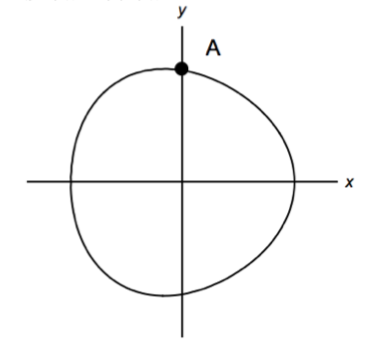
\includegraphics[scale=0.3]{Figures/curvec}
  \end{center}
\begin{enumerate}[(a)]
\item Find the coordinates $(x,y)$ of the point $A$.
\item Find $\displaystyle\frac{dy}{dx}$. 
\item Find the equation of tangent line $L(x)$ to the graph of $\mathcal{C}$ at $A$.

Show your computations step by step.
	\end{enumerate}
	\end{multicols}
        \begin{solution}
          See \href{https://dhsp.math.lsa.umich.edu/exams/115exam2/f17/s8.pdf}{https://dhsp.math.lsa.umich.edu/exams/115exam2/f17/s8.pdf}
        \end{solution}
\question A {\it quadrifolium} is a $4$-petaled rose curve given by
\begin{equation*}
	\big(x^2+y^2\big)^3=4x^2y^2
\end{equation*}
and which is shown below as the solid curve. It lies inside the unit
circle $x^2+y^2=1$.
%\footnote{Fun fact: quite surprisingly the area of the quadrifolium equals $\frac{\pi}{2}$\,!}
\begin{figure}[h]
\centering
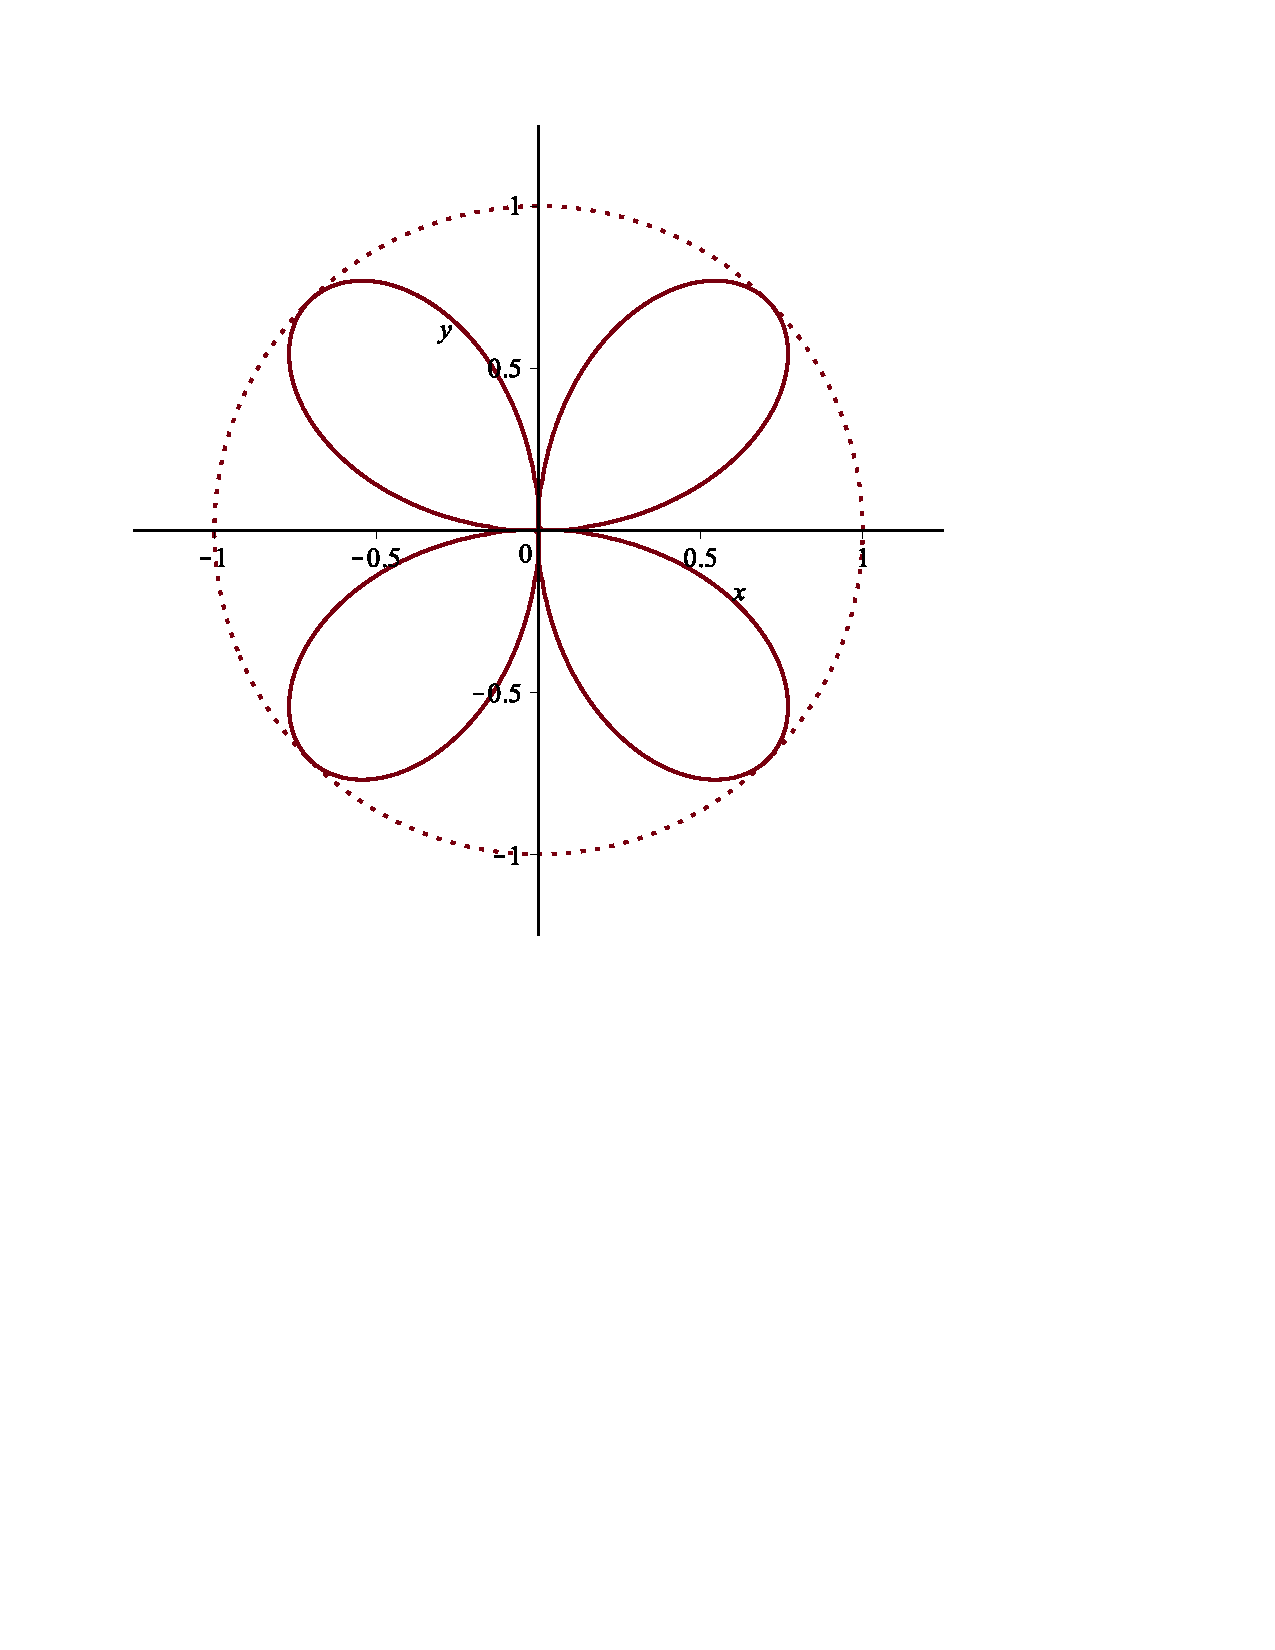
\includegraphics[width=10cm,height=10cm]{Figures/fig3.pdf}
\end{figure}
\begin{enumerate}[(a)]
	\item Show that the point $(x,y)=(\frac{1}{\sqrt{2}},\frac{1}{\sqrt{2}})$ lies on the quadrifolium.
	\item Find the equation of the tangent line to the quadrifolium at $(x,y)=(\frac{1}{\sqrt{2}},\frac{1}{\sqrt{2}})$.
\end{enumerate}
\begin{solution}
  \begin{enumerate}[(a)]
  \item We verify \[
      \left(\left(\frac{1}{\sqrt{2}}\right)^2+\left(\frac{1}{\sqrt{2}}\right)^2\right)^3 = 1^3 = 1 =
      4\cdot \frac{1}{2} \cdot \frac{1}{2} = 4
      \left(\frac{1}{\sqrt{2}} \right)^2
      \left(\frac{1}{\sqrt{2}} \right)^2
    \]
  \item We first differentiate with respect to \(x\) to get
    \begin{align*}
      3(x^2+y^2)^2 \left(2x+2y\dydx\right) = 8xy^2+8x^2y\dydx
      & \implies (2y\cdot 3(x^2+y^2)^2-8x^2y) \dydx = 8xy^2-3(2x)(x^2+y^2)^2 \\
      & \implies \dydx =\frac{8xy^2-6x(x^2+y^2)^2}{6y(x^2+y^2)^2-8x^2y} 
    \end{align*}
    If we plug in our point \(\left( \frac{1}{\sqrt{2}},
      \frac{1}{\sqrt{2}} \right)\) and observe that \(\left( \left(
        \frac{1}{\sqrt{2}} \right)^2+\left( \frac{1}{\sqrt{2}}
      \right)^2 \right) = 1\), we get
    \begin{align*}
      \dydx|_{\left( \frac{1}{\sqrt{2}},\frac{1}{\sqrt{2}} \right)}
      & =
      \frac{\frac{8}{2^{3/2}}-\frac{6}{2^{1/2}} \cdot 1}{\frac{6}{2^{1/2}}\cdot 1 -
      \frac{8}{2^{3/2}}} \\
      & = \frac{8/2-6}{6-8/2}\\
      & = \frac{4-6}{6-4} \\
      & = -1
    \end{align*}
  \end{enumerate}
\end{solution}
\pagebreak
\question (Winter 2018 Exam 2)
	Each the following is the graph of an implicit function.
\begin{multicols}{3}
  \begin{center}
    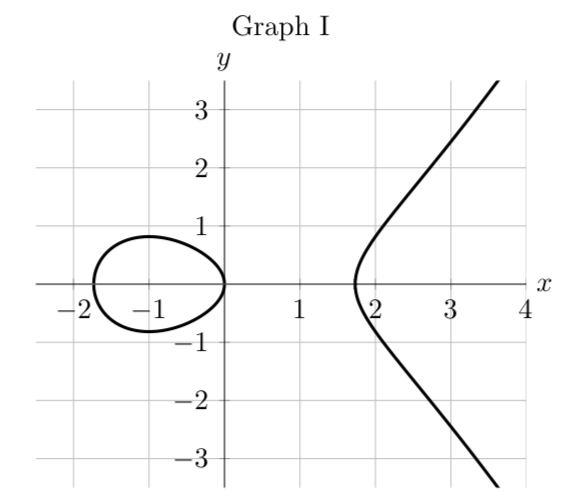
\includegraphics[scale=0.3]{Figures/graphI.png}
  \end{center}
  \begin{center}
    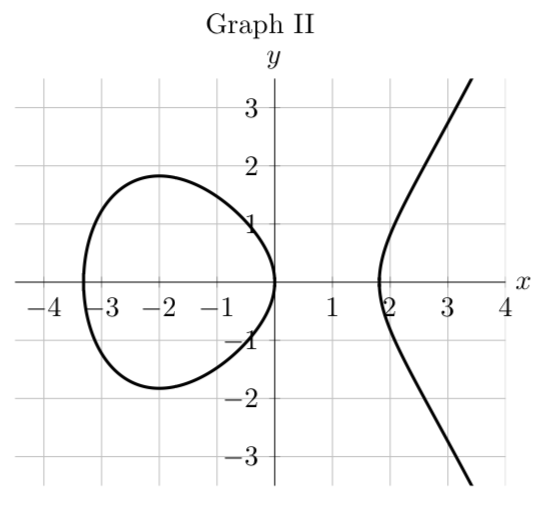
\includegraphics[scale=0.3]{Figures/graphII.png}
  \end{center}
  \begin{center}
    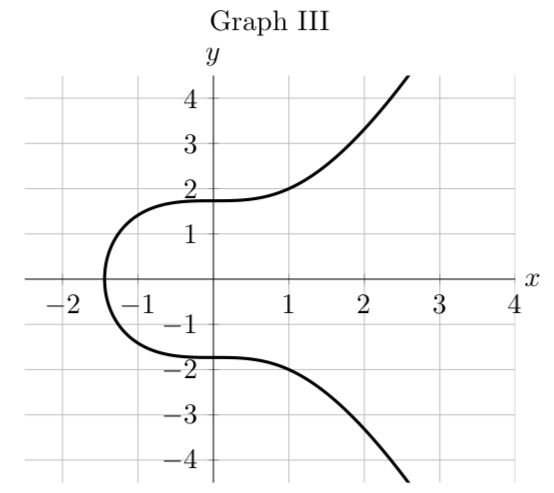
\includegraphics[scale=0.3]{Figures/graphIII.png}
  \end{center}
\end{multicols}
Match each of the graphs above to the formula below that gives the slope at each point on the graph.
\begin{multicols}{2}
\begin{enumerate}[(a)]
\item $\displaystyle\frac{dy}{dx} =\frac{3x^2}{2y}$
\item $\displaystyle\frac{dy}{dx} =\frac{(x-1)(x+2)}{2y}$
\item $\displaystyle\frac{dy}{dx} =\frac{x^2-1}{2y}$
\item $\displaystyle\frac{dy}{dx} =\frac{(y-1)(y+2)}{2x}$
\end{enumerate}
\end{multicols}
\begin{solution}
  See part (a) of \href{https://dhsp.math.lsa.umich.edu/exams/115exam2/w18/s2.pdf}{https://dhsp.math.lsa.umich.edu/exams/115exam2/w18/s2.pdf} 
\end{solution}
\end{questions}
\end{document}
%%% Local Variables:
%%% mode: latex
%%% TeX-master: t
%%% End:
